
\subsection*{4.1 Trigonometric Ratios and identities}
Trigonometric ratios relate the angles and sides of right-angled triangles. The three primary trigonometric functions are sine, cosine, and tangent.

\textbf{Key Concepts:}

\begin{itemize}
	\item \textbf{Right-Angled Triangle Definition:}
	In a right-angled triangle, the three sides are:
	\begin{itemize}
		\item Hypotenuse: The longest side, opposite the right angle.
		\item Opposite Side: The side opposite to the given angle.
		\item Adjacent Side: The side next to the given angle (excluding the hypotenuse).
	\end{itemize}
	
	\item \textbf{Trigonometric Ratios:}
	The three basic trigonometric ratios for an angle $\theta$ in a right-angled triangle are:
	\[
	\sin \theta = \frac{\text{opposite}}{\text{hypotenuse}}
	\]
	\[
	\cos \theta = \frac{\text{adjacent}}{\text{hypotenuse}}
	\]
	\[
	\tan \theta = \frac{\text{opposite}}{\text{adjacent}}
	\]
	
	
	\begin{center}
		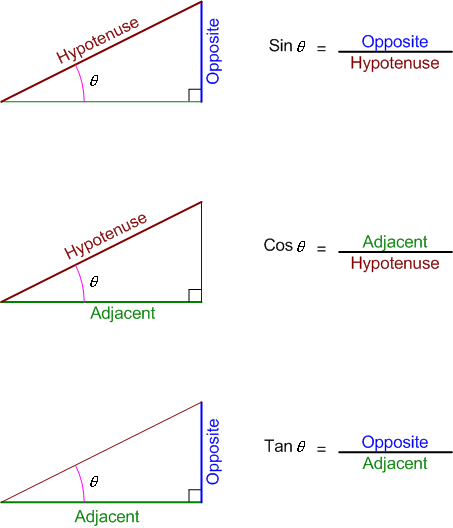
\includegraphics[width=0.6\textwidth]{4.1.png}
	\end{center}
	
	\newpage
	\item \textbf{Common Trigonometric Values:}
	\[
	\begin{array}{c|c|c|c}
		\theta & \sin \theta & \cos \theta & \tan \theta \\
		\hline
		0^\circ & 0 & 1 & 0 \\
		30^\circ & \frac{1}{2} & \frac{\sqrt{3}}{2} & \frac{1}{\sqrt{3}} \\
		45^\circ & \frac{\sqrt{2}}{2} & \frac{\sqrt{2}}{2} & 1 \\
		60^\circ & \frac{\sqrt{3}}{2} & \frac{1}{2} & \sqrt{3} \\
		90^\circ & 1 & 0 & \text{undefined} \\
	\end{array}
	\]
	
	\item \textbf{Reciprocal Trigonometric Functions:}
	\begin{itemize}
		\item Cosecant: $\csc \theta = \frac{1}{\sin \theta}$
		\item Secant: $\sec \theta = \frac{1}{\cos \theta}$
		\item Cotangent: $\cot \theta = \frac{1}{\tan \theta}$
	\end{itemize}
	
	\item \textbf{Pythagorean Identity:}
	\[
	\sin^2 \theta + \cos^2 \theta = 1.
	\]
\end{itemize}

\textbf{Examples:}

\begin{flushleft}
	\textbf{Example 1: Given a right-angled triangle where $\theta = 30^\circ$ and the hypotenuse is $10$ cm, find the opposite and adjacent sides.}
	
	\vspace{0.5cm}
	\textbf{Solution:}
	\vspace{0.5cm}
	
	Step 1: Use trigonometric ratios:
	\[
	\sin 30^\circ = \frac{\text{opposite}}{\text{hypotenuse}}.
	\]
	
	Substituting values:
	\[
	\frac{x}{10} = \frac{1}{2}.
	\]
	
	Solving for $x$:
	\[
	x = 10 \times \frac{1}{2} = 5 \text{ cm}.
	\]
	
	Step 2: Use the cosine function for the adjacent side:
	\[
	\cos 30^\circ = \frac{\text{adjacent}}{\text{hypotenuse}}.
	\]
	
	\[
	\frac{y}{10} = \frac{\sqrt{3}}{2}.
	\]
	
	Solving for $y$:
	\[
	y = 10 \times \frac{\sqrt{3}}{2} = 5\sqrt{3} \text{ cm}.
	\]
	
	Thus, the opposite side is $5$ cm, and the adjacent side is $5\sqrt{3}$ cm.
\end{flushleft}

\begin{flushleft}
	\textbf{Example 2: A ladder is leaning against a vertical wall. The foot of the ladder is $4$ m from the base of the wall, and the ladder makes an angle of $60^\circ$ with the ground. Find the length of the ladder.}
	
	\vspace{0.5cm}
	\textbf{Solution:}
	\vspace{0.5cm}
	
	Step 1: Identify the known values:
	- The adjacent side (distance from the wall) is $4$ m.
	- The hypotenuse is the length of the ladder.
	- The angle given is $60^\circ$.
	
	Step 2: Use the cosine function:
	\[
	\cos 60^\circ = \frac{\text{adjacent}}{\text{hypotenuse}}.
	\]
	
	\[
	\frac{4}{h} = \frac{1}{2}.
	\]
	
	Step 3: Solve for $h$:
	\[
	h = \frac{4}{\frac{1}{2}} = 8 \text{ m}.
	\]
	
	Thus, the ladder is $8$ m long.
\end{flushleft}

\begin{flushleft}
	\textbf{Example 3: Find $\tan \theta$ if $\sin \theta = 0.6$.}
	
	\vspace{0.5cm}
	\textbf{Solution:}
	\vspace{0.5cm}
	
	Step 1: Use the Pythagorean identity:
	\[
	\sin^2 \theta + \cos^2 \theta = 1.
	\]
	
	Substituting $\sin \theta = 0.6$:
	\[
	(0.6)^2 + \cos^2 \theta = 1.
	\]
	
	\[
	0.36 + \cos^2 \theta = 1.
	\]
	
	\[
	\cos^2 \theta = 0.64.
	\]
	
	\[
	\cos \theta = 0.8.
	\]
	
	Step 2: Use the tangent formula:
	\[
	\tan \theta = \frac{\sin \theta}{\cos \theta}.
	\]
	
	\[
	\tan \theta = \frac{0.6}{0.8} = 0.75.
	\]
	
	Thus, $\tan \theta = 0.75$.
\end{flushleft}

\begin{flushleft}
	\textbf{Example 4: Given that $\cos x = \frac{12}{13}$, evaluate $\frac{1 - \tan x}{\tan x}$.}
	
	\vspace{0.5cm}
	\textbf{Solution:}
	\vspace{0.5cm}
	
	Step 1: Use the Pythagorean identity to find $\sin x$:
	\[
	\sin^2 x + \cos^2 x = 1.
	\]
	
	Substituting $\cos x = \frac{12}{13}$:
	\[
	\sin^2 x + \left(\frac{12}{13}\right)^2 = 1.
	\]
	
	\[
	\sin^2 x + \frac{144}{169} = 1.
	\]
	
	\[
	\sin^2 x = 1 - \frac{144}{169} = \frac{169}{169} - \frac{144}{169} = \frac{25}{169}.
	\]
	
	\[
	\sin x = \frac{5}{13}.
	\]
	
	Step 2: Calculate $\tan x$:
	\[
	\tan x = \frac{\sin x}{\cos x} = \frac{\frac{5}{13}}{\frac{12}{13}} = \frac{5}{12}.
	\]
	
	Step 3: Evaluate $\frac{1 - \tan x}{\tan x}$:
	\[
	\frac{1 - \frac{5}{12}}{\frac{5}{12}}.
	\]
	
	Simplify the numerator:
	\[
	1 - \frac{5}{12} = \frac{12}{12} - \frac{5}{12} = \frac{7}{12}.
	\]
	
	Now, divide:
	\[
	\frac{\frac{7}{12}}{\frac{5}{12}} = \frac{7}{12} \times \frac{12}{5} = \frac{7}{5}.
	\]
	
	Thus, the final answer is:
	\[
	\frac{7}{5} 
	\]
\end{flushleft}
